\chapter*{Preliminary Concepts}
\section{What is sequential decision making?}\label{sec:intro-sdm}
\begin{figure}
    \centering
    \begin{tikzpicture}[
        node distance=2.5cm,
        auto,
        thick,
        state/.style={circle, draw, fill=blue!20, minimum size=1.5cm, text centered},
        environment/.style={rectangle, draw, dashed, fill=blue!10, rounded corners, minimum width=4cm, minimum height=2cm, text centered},
        agent/.style={rectangle, draw, fill=orange!20, rounded corners, minimum width=2cm, minimum height=1.5cm, text centered},
        robot/.style={rectangle, draw, fill=green!20, rounded corners, minimum width=2cm, minimum height=1.5cm, text centered},
        decision_box/.style={rectangle, draw, dashed, fill=gray!10, minimum width=7.5cm, minimum height=3cm, text centered},
        arrow/.style={->, thick, bend left=15},
        arrow_decision/.style={->, dashed, bend left=15}
    ]
        
        % Decision Making Box
        \node[decision_box] (decision_box) at (0.3,3.4) {};
        \node at (0.3,4.5) {\small{Decision Making}};
        
        % Robot (AI)
        \node[robot] (robot) at (-2.1,3.2) {
            \begin{minipage}{1.5cm}
                \centering
                \includesvg[width=0.4cm]{images/images_intro/robot-svgrepo-com.svg}\\
                \small{Computer program}
            \end{minipage}
        };
        
        % Doctor
        \node[agent] (doctor) at (2.5,3.2) {
            \begin{minipage}{1.5cm}
                \centering
                \includesvg[width=0.4cm]{images/images_intro/doctor-with-stethoscope-svgrepo-com.svg}\\
                \small{Doctor}
            \end{minipage}
        };
        
        % Environment (Patient)
        \node[environment] (environment) at (0,-0.5) {
            \begin{minipage}{2cm}
                \centering
                \includesvg[width=0.8cm]{images/images_intro/patient-4.svg}\\
                \small{Cancer patient}
            \end{minipage}
        };
        
        % Arrows
        \draw[arrow] (environment) to[bend left=30] node[left] {
            \begin{minipage}{2cm}
                \centering
                \includesvg[width=0.4cm]{images/images_intro/patient-clipboard-svgrepo-com.svg}\\
                \small{Updated health status}
            \end{minipage}
        } (robot);
        \draw[arrow_decision] (robot) to node[above] {\small{Recommends}} (doctor);
        \draw[arrow_decision] (doctor) to node[below] {\small{Interprets}} (robot);

        \draw[arrow] (doctor) to[bend left=30] node[right] {
            \begin{minipage}{1.5cm}
                \centering
                \includesvg[width=0.5cm]{images/images_intro/syringe-svgrepo-com.svg}\\
                \small{Administer chemotherapy}
            \end{minipage}
        } (environment);
        
    \end{tikzpicture}
    \caption{Sequential decision making in cancer treatment. The AI system reacts to the patient's current state (tumor size, blood cells counts, etc.) and makes a recommendation to the doctor, who administers chemotherapy to the patient. The patient's state is then updated, and this cycle repeats over time.}
    \label{fig:cancer-treatment-sdm}
\end{figure}
In this manuscript, we study algorithms for sequential decision making. Humans engage in sequential decision making in all aspects of life. In medicine, doctors have to decide how much chemotherapy to administer based on the patient's current health~\cite{cancer}. In agriculture, agronomists have to decide when to fertilize based on the current soil and weather conditions to maximize plant growth~\cite{agriculture}. 
In automotive settings, the autopilot system has to decide how to steer based on lidar and other sensors to maintain a safe trajectory~\cite{driving}. 
These sequential decision making processes exhibit key similarities: an agent takes actions based on current information to achieve a goal.

As computer scientists, we ought to design computer programs~\cite{knuth63} that can help humans during these sequential decision making processes. 
For example, as depicted in figure~\ref{fig:cancer-treatment-sdm}, a doctor could benefit from a program that would recommend the ``best'' treatment given the patient's state. 
Machine learning algorithms~\cite{turing} output such helpful programs.
For non-sequential decision making, when the doctor only takes one decision and does not need to react to the updated patient's health, e.g. making a diagnosis about cancer type, a program can be fitted to example data: given lots of patient records and the associated diagnoses, the program learns to make the same diagnosis a doctor would given the same patient record, this is \textit{supervised} learning~\cite{sl}. 
In the cancer treatment example, the doctor follows the patient over time and adapts treatment to the patient's changing health. In that case, machine learning—and in particular \textit{reinforcement} learning (RL)~\cite{sutton}—can be used to teach the program how to take decisions that lead to recovery based on how the patient's health changes from one dose to another.  
Such machine learning algorithms train increasingly performant programs that are deployed to, e.g., identify digits in images~\cite{lenet}, control tokamak fusion~\cite{tokamak}, or write the abstract of a scientific article~\cite{reinforce-llm}.

However, the computations performed by these programs cannot be understood and verified by humans: the programs are black-box.
This can be problematic in applications where decisions have important consequences. 
Consider the following extreme scenario in the context of the cancer treatment example: a program recommends to the doctor to amputate a patient's limb.
While amputating could be the only way to save the patient's life, it is not hard to imagine that such an extreme recommendation would not be followed by the doctor unless it comes with convincing explanations or unless the factors that influenced the program's recommendation can be presented to the doctor. 
In an other setting where the program directly act in the real-world, i.e. it does not make recommendations to a human but rather acts autonomously, black-box programs are also not desirable.
Consider the slightly extreme scenario of a combat drone in which a program decides on who to shoot.
In this context, it is hard to imagine leaders deploying such drones and programs without having strict guarantees that it will, e.g. not shoot civilians.
Such guarantees can be obtained through formal verifications of programs which in turn can only be obtain for certain programs.

Next, we describe the notion of interpretability that is key to ensure that programs can be verified and their recommendations can be understood.

\section{What is Interpretability?}


Originally, the etymology of ``interpretability'' is the Latin ``interpretabilis'', meaning ``that can be understood and explained''.
According to the Oxford English Dictionary, the first recorded use of the English word ``interpretability'' dates back to 1854, when the British logician George Boole (figure~\ref{fig:george-boole}) described the addition of concepts:

\begin{displaycquote}[p.~48]{boole}
I would remark in the first place that the generality of a method in Logic
must very much depend upon the generality of its elementary processes and laws.
We have, for instance, in the previous sections of this work investigated, among
other things, the laws of that logical process of addition which is symbolized by
the sign +. Now those laws have been determined from the study of instances,
in all of which it has been a necessary condition, that the classes or things added
together in thought should be mutually exclusive. The expression x + y seems
indeed uninterpretable, unless it be assumed that the things represented by x
and the things represented by y are entirely separate; that they embrace no
individuals in common. And conditions analogous to this have been involved
in those acts of conception from the study of which the laws of the other
symbolical operations have been ascertained. The question then arises, whether
it is necessary to restrict the application of these symbolical laws and processes
by the same conditions of interpretability under which the knowledge of them
was obtained. If such restriction is necessary, it is manifest that no such thing
as a general method in Logic is possible. On the other hand, if such restriction
is unnecessary, in what light are we to contemplate processes which appear to
be uninterpretable in that sphere of thought which they are designed to aid?
\end{displaycquote}\label{quote:boole}

\begin{figure}
    \centering
    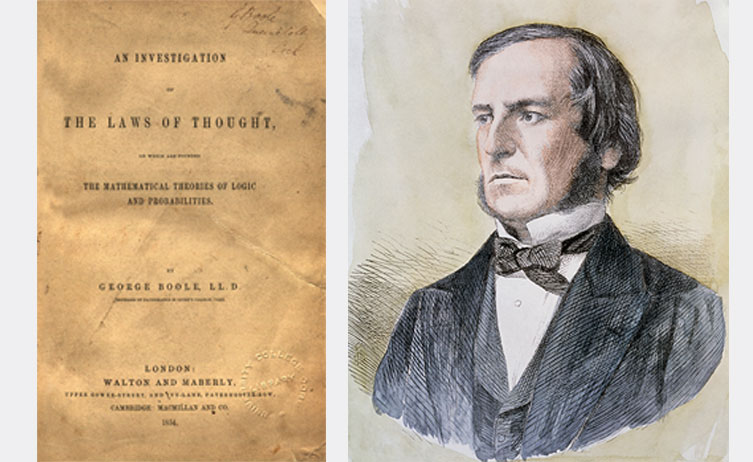
\includegraphics[width=0.5\textwidth]{images/images_intro/gboole.jpg}
    \caption{British logician and philosopher George Boole (1815--1864) next to his book \textit{The Laws of Thought} (1854), the oldest known record of the word ``interpretability''.}
    \label{fig:george-boole}
\end{figure}

What is remarkable is that the first recorded occurrence of ``interpretability'' was in the context of logic and computation. 
In Boole's system, the expression $x+y$ is interpretable only when $x$ and $y$ are disjoint sets, because then ``+'' clearly represents their union. 
By contrast, in e.g. a neural network program~\cite{perceptron}, an operation like $x+y$ typically means adding two hidden vectors in a high-dimensional space. 
The result is mathematically well-defined, but its semantic meaning—what concept or feature this new vector corresponds to—is black-box. 
Just as Boole worried that logic would lose its generality and practical use if restricted only to easily interpretable operations, there exists similar tension in machine learning today.
In machine learning, should we limit ourselves to inherently interpretable programs (like decision trees~\cite{breiman1984classification}, where $x+y$ might literally mean combining two feature contributions, like blood cells count and tumor size) or accept uninterpretable computations in black-box programs (like in neural networks) in order to have broadly applicable and highly performant programs?
The global trend in machine learning research answers the latter.

\begin{figure}
    \centering
    \begin{subfigure}[b]{0.7\textwidth}
        \centering
        \begin{tikzpicture}[
            node distance=2.5cm,
            auto,
            thick,
            state/.style={circle, draw, fill=blue!20, minimum size=1.5cm, text centered},
            environment/.style={rectangle, draw, dashed, fill=blue!10, rounded corners, minimum width=4cm, minimum height=2cm, text centered},
            agent/.style={rectangle, draw, fill=orange!20, rounded corners, minimum width=2cm, minimum height=1.5cm, text centered},
            robot/.style={rectangle, draw, fill=black!20, rounded corners, minimum width=2cm, minimum height=1.5cm, text centered},
            ml/.style={circle, draw, fill=purple!20, minimum width=2cm, minimum height=1cm, text centered},
            decision_box/.style={rectangle, draw, dashed, fill=gray!10, minimum width=7.5cm, minimum height=3cm, text centered},
            arrow/.style={->, thick, bend left=15},
            arrow_decision/.style={->, dashed, bend left=15}
        ]
            
            % Decision Making Box
            \node[decision_box] (decision_box) at (0.3,3.4) {};
            \node at (0.3,4.5) {\small{Decision Making}};
            
            % Robot (AI)
            \node[robot] (robot) at (-2.1,3.2) {
                \begin{minipage}{1.5cm}
                    \centering
                    \includesvg[width=0.4cm]{images/images_intro/network-mapping-svgrepo-com.svg}\\
                    \small{Neural network}
                \end{minipage}
            };
            
            % Doctor
            \node[agent] (doctor) at (2.5,3.2) {
                \begin{minipage}{1.5cm}
                    \centering
                    \includesvg[width=0.4cm]{images/images_intro/doctor-with-stethoscope-svgrepo-com.svg}\\
                    \small{Doctor}
                \end{minipage}
            };
            
            % Machine Learning component
            \node[ml] (ml) at (-7,3) {
                \begin{minipage}{1.8cm}
                    \centering
                    \includesvg[width=0.4cm]{images/images_intro/gear-file-svgrepo-com.svg}\\
                    \small{Machine learning}
                \end{minipage}
            };
            
            % Environment (Patient)
            \node[environment] (environment) at (0,-0.5) {
                \begin{minipage}{2cm}
                    \centering
                    \includesvg[width=0.8cm]{images/images_intro/patient-4.svg}\\
                    \small{Cancer patient}
                \end{minipage}
            };
            
            % Arrows
            \draw[arrow] (environment) to[bend left=30] node[left] {
                \begin{minipage}{2cm}
                    \centering
                    \includesvg[width=0.5cm]{images/images_intro/patient-clipboard-svgrepo-com.svg}\\
                    \small{Updated health status}
                \end{minipage}
            } (robot);
            \draw[arrow_decision] (robot) to node[above] {\small{Recommends}} (doctor);
            \draw[arrow_decision, red] (doctor) to node[below] {\small{Cannot interpret}} (robot);
            
        \draw[arrow] (doctor) to[bend left=30] node[right] {
                \begin{minipage}{1.5cm}
                    \centering
                    \includesvg[width=0.5cm]{images/images_intro/syringe-svgrepo-com.svg}\\
                \small{Administer chemotherapy}
                \end{minipage}
            } (environment);
            
            % ML learning arrows
            \draw[arrow] (environment) to[bend left=40] node[left] {
                \begin{minipage}{2cm}
                    \centering
                    \includesvg[width=0.5cm]{images/images_intro/patient-clipboard-svgrepo-com.svg}\\
                    \small{Treatment outcomes}
                \end{minipage}
            } (ml);
            \draw[arrow] (ml) to[bend left=20] node[above] {
                \begin{minipage}{1.5cm}
                    \centering
                    \small{Updates program}
                \end{minipage}
            } (robot);
            
        \end{tikzpicture}
        \caption{Black-box approach using neural networks}
        \label{fig:cancer-treatment-sdm-ml}
    \end{subfigure}
    
    \vspace*{1cm}
    
    \begin{subfigure}[b]{0.7\textwidth}
        \centering
        \begin{tikzpicture}[
            node distance=2.5cm,
            auto,
            thick,
            state/.style={circle, draw, fill=blue!20, minimum size=1.5cm, text centered},
            environment/.style={rectangle, draw, dashed, fill=blue!10, rounded corners, minimum width=4cm, minimum height=2cm, text centered},
            agent/.style={rectangle, draw, fill=orange!20, rounded corners, minimum width=2cm, minimum height=1.5cm, text centered},
            robot/.style={rectangle, draw, fill=green!20, rounded corners, minimum width=2cm, minimum height=1.5cm, text centered},
            ml/.style={circle, draw, fill=purple!20, minimum width=2cm, minimum height=1cm, text centered},
            decision_box/.style={rectangle, draw, dashed, fill=gray!10, minimum width=7.5cm, minimum height=3cm, text centered},
            arrow/.style={->, thick, bend left=15},
            arrow_decision/.style={->, dashed, bend left=15}
        ]
            
            % Decision Making Box
            \node[decision_box] (decision_box) at (0.3,3.4) {};
            \node at (0.3,4.5) {\small{Decision Making}};
            
            % Robot (AI)
            \node[robot] (robot) at (-2.1,3.2) {
                \begin{minipage}{1.5cm}
                    \centering
                    \includesvg[width=0.4cm]{images/images_intro/decision-tree-svgrepo-com.svg}\\
                    \small{Decision tree}
                \end{minipage}
            };
            
            % Doctor
            \node[agent] (doctor) at (2.5,3.2) {
                \begin{minipage}{1.5cm}
                    \centering
                    \includesvg[width=0.4cm]{images/images_intro/doctor-with-stethoscope-svgrepo-com.svg}\\
                    \small{Doctor}
                \end{minipage}
            };
            
            % Machine Learning component
            \node[ml] (ml) at (-7,3) {
                \begin{minipage}{1.8cm}
                    \centering
                    \includesvg[width=0.4cm]{images/images_intro/gear-file-svgrepo-com.svg}\\
                    \small{Interpretable machine learning}
                \end{minipage}
            };
            
            % Environment (Patient)
            \node[environment] (environment) at (0,-0.5) {
                \begin{minipage}{2cm}
                    \centering
                    \includesvg[width=0.8cm]{images/images_intro/patient-4.svg}\\
                    \small{Cancer patient}
                \end{minipage}
            };
            
            % Arrows
            \draw[arrow] (environment) to[bend left=30] node[left] {
                \begin{minipage}{2cm}
                    \centering
                    \includesvg[width=0.5cm]{images/images_intro/patient-clipboard-svgrepo-com.svg}\\
                    \small{Updated health status}
                \end{minipage}
            } (robot);
            \draw[arrow_decision] (robot) to node[above] {\small{Recommends}} (doctor);
            \draw[arrow_decision, green] (doctor) to node[below] {\small{Can interpret}} (robot);
            
            \draw[arrow] (doctor) to[bend left=30] node[right] {
                \begin{minipage}{1.5cm}
                    \centering
                    \includesvg[width=0.5cm]{images/images_intro/syringe-svgrepo-com.svg}\\
                    \small{Administer chemotherapy}
                \end{minipage}
            } (environment);
            
            % ML learning arrows
            \draw[arrow] (environment) to[bend left=40] node[left] {
                \begin{minipage}{2cm}
                    \centering
                    \includesvg[width=0.5cm]{images/images_intro/patient-clipboard-svgrepo-com.svg}\\
                    \small{Treatment outcomes}
                \end{minipage}
            } (ml);
            \draw[arrow] (ml) to[bend left=20] node[above] {
                \begin{minipage}{1.5cm}
                    \centering
                    \small{Updates program}
                \end{minipage}
            } (robot);
            
        \end{tikzpicture}
        \caption{Interpretable approach using decision trees}
        \label{fig:cancer-treatment-comparison}
    \end{subfigure}
    \caption{Comparison of sequential decision making approaches in cancer treatment. Top: a black-box neural network approach where the doctor cannot interpret the AI's recommendations because the computations are operations over uninterpretable concepts (cf. end of section~\ref{sec:intro-sdm} and Boole's quote~\ref{quote:boole}). Bottom: an interpretable decision tree approach where the doctor can understand and verify the AI's recommendations because the operations are performed over meaningful concepts  (cf. end of section~\ref{sec:intro-sdm} and Boole's quote~\ref{quote:boole}). Both systems learn from treatment outcomes to improve their recommendations over time.}
    \label{fig:cancer-treatment-comparison-combined}
\end{figure}

In figure~\ref{fig:cancer-treatment-sdm-ml}, we illustrate how existing machine learning algorithms \textit{could} be used in principle to help with cancer treatment. In truth, this should be prohibited without some kind of transparency in the program's recommendation: why did the program recommend such a dosage?
In figure~\ref{fig:cancer-treatment-comparison}, we illustrate how machine learning \textit{should} be used in practice. 
Ideally, we want doctors to have access to computer programs that can recommend ``good'' treatments and whose recommendations are interpretable. 
In the next section, present related works that fit this desiderata.

\section{What are existing approaches for learning interpretable programs?}\label{sec:intro-interp}

In this section we follow sections 6 and 7 of \cite{glanois-survey} and section 5 of \cite{milani-survey}. 
Furthermore we now employ the term ``model'' to refer to ``programs'' to be consistent with the machine learning research conventions.
Models are essentially mappings from inputs to outputs that can be trained with machine learning algorithms while programs might designate other types of computations like \texttt{print("Hello World");}.

\begin{figure}
    \centering
    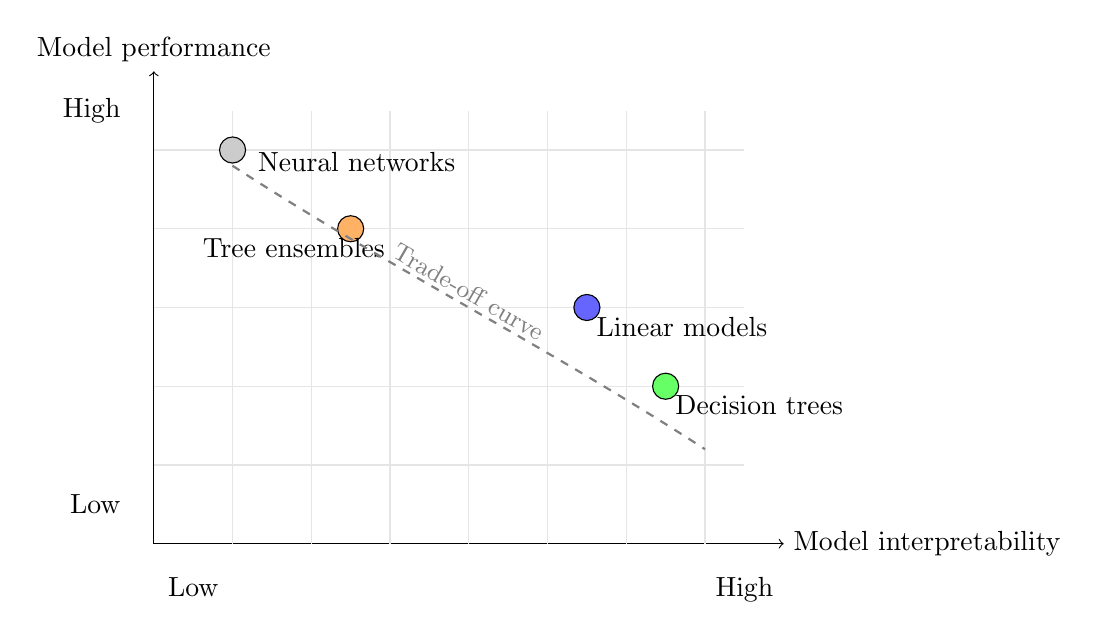
\begin{tikzpicture}
        % Define the axes
        \draw[->] (0,0) -- (8,0) node[right] {Model interpretability};
        \draw[->] (0,0) -- (0,6) node[above] {Model performance};
        
        % Add axis labels at the ends
        \node[below] at (0.5,-0.3) {Low};
        \node[below] at (7.5,-0.3) {High};
        \node[left] at (-0.3,0.5) {Low};
        \node[left] at (-0.3,5.5) {High};
        
        % Add grid lines (optional, subtle)
        \foreach \x in {1,2,...,7}
            \draw[gray!20] (\x,0) -- (\x,5.5);
        \foreach \y in {1,2,...,5}
            \draw[gray!20] (0,\y) -- (7.5,\y);
            
        % Position different model types
        % Deep Neural Networks (high performance, low interpretability)
        \node[circle, fill=black!20, draw, minimum size=8pt] at (1,5) {};
        \node[below right] at (1.2,5.1) {Neural networks};
        
        % Ensemble Methods (medium-high performance, low-medium interpretability)
        \node[circle, fill=orange!60, draw, minimum size=8pt] at (2.5,4) {};
        \node[below right] at (0.5,4) {Tree ensembles};
        
        % Linear Models (medium performance, high interpretability)
        \node[circle, fill=blue!60, draw, minimum size=8pt] at (5.5,3) {};
        \node[below right] at (5.5,3) {Linear models};
        
        % Decision Trees (medium-low performance, high interpretability)
        \node[circle, fill=green!60, draw, minimum size=8pt] at (6.5,2) {};
        \node[below right] at (6.5,2) {Decision trees};
        

        
        % Add a general trend line (optional)
        \draw[dashed, thick, gray] (1,4.8) .. controls (3,3.5) and (5,2.5) .. (7,1.2);
        \node[gray, rotate=-30] at (4,3.2) {\small Trade-off curve};
        
    \end{tikzpicture}
    \caption{The interpretability–performance trade-off in machine learning. Different model classes are positioned according to their typical interpretability and performance characteristics. The dashed line illustrates the general trade-off between these two properties.}
    \label{fig:interpretability-performance-tradeoff}
\end{figure}
Interpretable machine learning provides either local or global interpretations \cite{glanois-survey}.
Global methods, like decision tree induction~\cite{breiman1984classification}, return a model whose outputs can be interpreted without having to run an additional algorithm.
By contrast, local methods require to run an additional algorithm, e.g. linear regression~\cite{regression}, but are agnostic to the model class.
In figure~\ref{fig:interpretability-performance-tradeoff} we present a popular trade-off between interpretability and performance of different model classes based on various user studies and popular beliefs~\cite{study-0,study-1,study-2,study-3,study-4,study-5,study-6,study-7}.

Local interpretable model-agnostic explanations (LIME)~\cite{lime} is a popular local interpretability method.
Given a model, LIME works by perturbing the input and learning a simple interpretable model locally to explain that particular prediction (see figure~\ref{fig:lime}). 
For each individual prediction, LIME provides interpretations by identifying which features were most important for that specific decision.

Local interpretability can also be called explainability.
Global interpretability methods constrain the model class so that the computations are transparent or verifiable by construction. 
On the other hand, explainability methods--or local interpretability methods--keep black-box models and generates post hoc explanations of their decisions. 
In additions to linear models, explanations can take various forms: visual explanations with saliency maps \cite{Puri2020Explain}, attribution such as SHAP\cite{shap}, attention-based highlighting \cite{attention}.

While useful for insight, these explanations are often subjective and might not be faithful to the underlying computations~\cite{Atrey2020Exploratory}.
For safety-critical settings, this motivates our focus on models that are interpretable by design.
Those interpretable by design models can be obtained by global interpretability methods that we present next.

\begin{figure}
    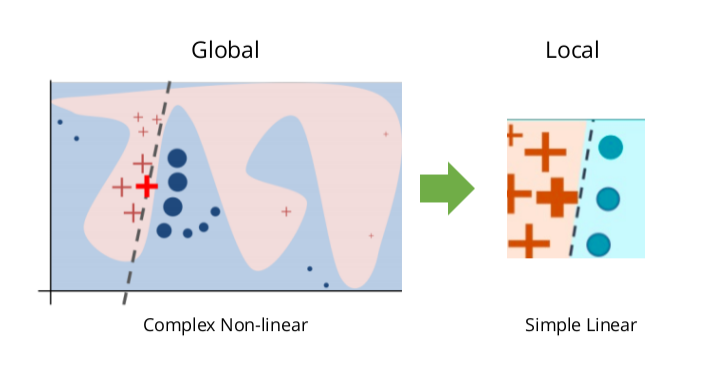
\includegraphics[width=0.9\textwidth]{images/lime.png}
    \caption{Local Interpretable Model-agnostic Explanations~\cite{lime} fit an interpretable linear model to data around the red cross prediction to be interpreted.}\label{fig:lime}
\end{figure}


\begin{figure}
    \centering
    \begin{tikzpicture}[
        node distance=2cm,
        auto,
        thick,
        rl/.style={circle, draw, fill=purple!20, minimum width=1.5cm, minimum height=0.8cm, text centered},
        nn/.style={rectangle, draw, fill=black!20, rounded corners, minimum width=1.5cm, minimum height=1cm, text centered},
        sl/.style={circle, draw, fill=blue!20, minimum width=1.5cm, minimum height=0.8cm, text centered},
        dt/.style={rectangle, draw, fill=green!20, rounded corners, minimum width=1.5cm, minimum height=1cm, text centered},
        arrow/.style={->, thick},
        label/.style={font=\tiny, above},
        method_box/.style={rectangle, draw, dashed, minimum width=5cm, minimum height=3cm, text centered},
        method_box_indirect/.style={rectangle, draw, dashed, minimum width=9.5cm, minimum height=3cm, text centered}
    ]
        
        % Direct method box
        \node[method_box] (direct_box) at (-0.5,0) {};
        \node at (-0.5,1.7) {\small{Direct}};
        
        % Direct method - RL process
        \node[rl] (rl_direct) at (-2,0) {
            \begin{minipage}{1.2cm}
                \centering
                \includesvg[width=0.3cm]{images/images_intro/gear-file-svgrepo-com.svg}\\
                \tiny{Reinforcement learning}
            \end{minipage}
        };
        
        % Direct method - Decision Tree
        \node[dt] (dt_direct) at (1,0) {
            \begin{minipage}{1.2cm}
                \centering
                \includesvg[width=0.3cm]{images/images_intro/decision-tree-svgrepo-com.svg}\\
                \tiny{Decision tree}
            \end{minipage}
        };
        
        % Direct method arrow
        \draw[arrow] (rl_direct) -- (dt_direct) node[label, midway] {\tiny Learns};
        
        % Indirect method box
        \node[method_box_indirect] (indirect_box) at (7.1,0) {};
        \node at (6.8,1.7) {\small{Indirect}};
        
        % Indirect method - RL process
        \node[rl] (rl_indirect) at (3.5,0) {
            \begin{minipage}{1.2cm}
                \centering
                \includesvg[width=0.3cm]{images/images_intro/gear-file-svgrepo-com.svg}\\
                \tiny{Reinforcement learning}
            \end{minipage}
        };
        
        % Indirect method - Neural Network
        \node[nn] (nn_indirect) at (6,0) {
            \begin{minipage}{1.2cm}
                \centering
                \includesvg[width=0.3cm]{images/images_intro/network-mapping-svgrepo-com.svg}\\
                \tiny{Neural network}
            \end{minipage}
        };
        
        % Indirect method - Supervised Learning
        \node[sl] (sl_indirect) at (8.5,0) {
            \begin{minipage}{1.2cm}
                \centering
                \includesvg[width=0.3cm]{images/images_intro/gear-file-svgrepo-com.svg}\\
                \tiny{Supervised learning}
            \end{minipage}
        };
        
        % Indirect method - Decision Tree
        \node[dt] (dt_indirect) at (11,0) {
            \begin{minipage}{1.2cm}
                \centering
                \includesvg[width=0.3cm]{images/images_intro/decision-tree-svgrepo-com.svg}\\
                \tiny{Decision Tree}
            \end{minipage}
        };
        
        % Indirect method arrows
        \draw[arrow] (rl_indirect) -- (nn_indirect) node[label, midway] {\tiny Learns};
        \draw[arrow] (nn_indirect) -- (sl_indirect) node[label, midway] {\tiny Generates data};
        \draw[arrow] (sl_indirect) -- (dt_indirect) node[label, midway] {\tiny Learns};
        
    \end{tikzpicture}
    \caption{Comparison of direct and indirect approaches for learning interpretable models in sequential decision making.}
    \label{fig:direct-vs-indirect-methods}
\end{figure}

Global approaches are either direct or indirect~\cite{milani-survey}. 
Direct algorithms, such as decision tree induction~\cite{breiman1984classification}, \textit{directly} learn an interpretable model optimizing some objective (see figure~\ref{fig:interpretability-performance-tradeoff}).
One key challenge motivating this thesis is that decision tree induction is well-developed for supervised learning but not for reinforcement learning.
To directly learn interpretable models for sequential decision making, one must design new algorithms which will be the core of the first part of this thesis. 

Most existing research has focused on developing indirect methods. 
Indirect methods for interpretable sequential decision making—sometimes called \textit{post hoc} methods—begin by learning a non-interpretable model (e.g., reinforcement learning of a neural network model), and then use supervised learning to fit an interpretable model that emulates the black-box.
Indirect methods rely on behavior cloning or imitation learning~\cite{behavior-cloning,dagger} to emulate the black-box models.
Most work on interpretable sequential decision focuses on the indirect approach\cite{viper,PIRL}.

Verifiable Reinforcement learning via Policy Extraction, or VIPER \cite{viper}, is a strong indirect method to learn decision tree models for sequential decision making. VIPER first trains a neural network model with reinforcement learning and then fit a decision tree to minimize the disagreement between the neural network and the tree outputs given the same inputs.
They show that decision tree models, in addition to being transparent, are also fast to verify in the formal sense of the term \cite{maraboupy}.
Programmatic models are an interpretable class that contains decision trees. 
Programmatically Interpretable Reinforcement Learning (PIRL) \cite{PIRL} synthesizes programs in a domain-specific language, also by imitating a neural network model. 

However, unlike direct methods that return interpretable models optimizing the desired objective, indirect methods learn an interpretable model to match the behavior of a black-box that itself optimizes the objective of interest. 
Due to the restricted policy class, the best decision tree model might employ a completely different strategy than the best black-box neural network model to solve the task.
Furthermore, the decision tree model that best fits the best neural network model might be sub-optimal compared to the decision tree model that best solves the task of interest.
Hence, there is no guarantee that optimizing this surrogate objective of best emulating a black-box yields the best interpretability–performance trade-offs. 
Figure~\ref{fig:direct-vs-indirect-methods} illustrates the key difference between these two approaches. 

Beyond direct and indirect learning, a complementary strategy is to train experts that are inherently easier to imitate and understand.
This is achieved by adding interpretability-oriented regularization during training. In the context of supervised learning tasks, authors of \cite{parbhoo} regularize the neural network model during training such that indirect approaches will be biased towards more interpretable trees.

In addition to finding models which computations can be read by humans or that can be formally verified, interpretable machine learning has also been used to detect reward misalignment in sequential decision making: by exposing the decision process of a model, one can identify goal mis-specification or unintended shortcuts.
Such shortcuts can be, for example, following the shadow of someone instead of actually following someone because for the model they lead to the same reactions.
The learning of interpretable models for misalignment detection has been heavily studied by Quentin Delfosse contemporarily to this manuscript \cite{scobots,shindo2024blendrl,nudge,ocatari}.
In the next chapter, we describe technical preliminaries useful to understand the content of this manuscript.

\chapter*{Technical preliminaries}\label{sec:technicals}

\section{What are decision trees?}\label{sec:dt}

As the reader might have already guessed, we will put great emphasis on decision tree models as a mean to study interpretability.
While other interpretable models might have other properties than the ones we will highlight through this thesis, one conjecture from \cite{glanois-survey} is that interpretable models are all hard to optimize or learn because they are non-differentiable in nature.
This is something that will be key in our study of decision tree models that we introduce next and that we illustrate in figure~\ref{fig:dt}.

\begin{definition}[Decision tree]
    A decision tree is a rooted tree $T = (\mathcal{N}, E)$ where:
    \begin{itemize}
    \item Each internal node $\nu \in \mathcal{N}$ is associated with a test that maps input features $x_{ij} \in \mathcal{X}$ to a Boolean.
    \item Each edge $e \in E$ from an internal node corresponds to an outcome of the associated test function.
    \item Each leaf node $l \in \mathcal{N}$ is associated with a prediction $y_l \in \mathcal{Y}$, where $\mathcal{Y}$ is the output space.
    \item For any input $x \in \mathcal{X}$, the tree defines a unique path from root to leaf, determining the prediction $T(x) = y_l$ where $l$ is the reached leaf.
    \end{itemize}
    The depth of a tree is the maximum path length from root to any leaf.
    \end{definition}

\begin{figure}
    \centering
    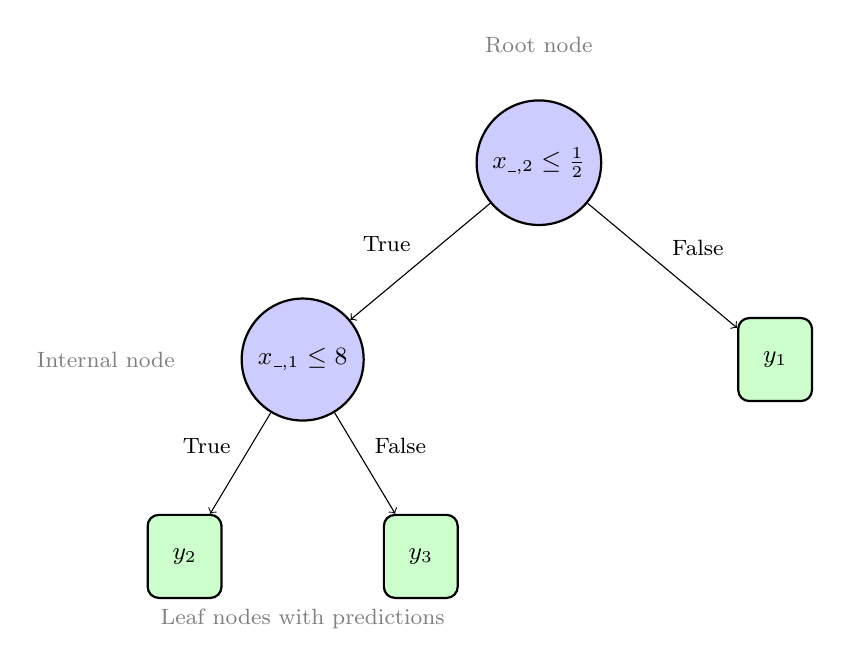
\begin{tikzpicture}[
        scale=1.0,
        decision/.style={circle, draw, thick, fill=blue!20, text width=3.5em, text centered, minimum height=3.5em, font=\small},
        leaf/.style={rectangle, draw, thick, fill=green!20, text width=2em, text centered, rounded corners, minimum height=3em, font=\small},
        edge_label/.style={font=\footnotesize, midway}
    ]
        % Root decision node
        \node[decision] (root) at (0,0) {$x_{\_, 2} \leq \frac{1}{2}$};
        
        % Second level nodes
        \node[decision] (left_decision) at (-3, -2.5) {$x_{\_, 1}\leq 8$};
        \node[leaf] (right_leaf) at (3, -2.5) {$y_1$};
        
        % Third level nodes (leaves)
        \node[leaf] (left_left) at (-4.5, -5) {$y_2$};
        \node[leaf] (left_right) at (-1.5, -5) {$y_3$};
        
        % Connections with labels
        \draw[->] (root) -- (left_decision) node[edge_label, above left] {True};
        \draw[->] (root) -- (right_leaf) node[edge_label, above right] {False};
        \draw[->] (left_decision) -- (left_left) node[edge_label, above left] {True};
        \draw[->] (left_decision) -- (left_right) node[edge_label, above right] {False};
        
        % Add labels for components
        \node[font=\footnotesize, text=gray] at (0, 1.5) {Root node};
        \node[font=\footnotesize, text=gray] at (-5.5, -2.5) {Internal node};
        \node[font=\footnotesize, text=gray] at (-3, -5.8) {Leaf nodes with predictions};
        
    \end{tikzpicture}
    \caption{A generic depth 2 decision tree with 2 nodes and 3 leaves. The root node applies the test $1_{\{x_{\_,1}\leq \frac{1}{2}\}}$ to check if the first features of data is below $\frac{1}{2}$. Edges represent the outcomes of the tests in each internal nodes(True/False), and leaf nodes contain predictions $y_l \in \mathcal{Y}$. For any input $\boldsymbol{x}_i$, the tree defines a unique path from root to leaf.}
    \label{fig:dt}
\end{figure}

\section{How to learn decision trees?}\label{sec:sl}
Training decision trees to optimize the following supervised learning objective is well studied~\cite{breiman1984classification}.

\begin{definition}[Supervised learning objective for classification or regression]\label{def:sl}
    Assume that we have access to a set of $N$ examples denoted $\mathcal{E} = {\{(\boldsymbol{x}_i, y_i)\}}_{i=1}^N$. Each datum $\boldsymbol{x}_i \in \mathcal{X}$ is described by a set of $p$ features $x_{ij}$ with $1\leq j \leq p $ . $y_i \in {\mathcal Y}$ is the label associated with $\boldsymbol{x}_i$.
    For a classification task $\mathcal{Y}=\{1,\ldots,K\}$ and for a regression task $\mathcal{Y}\subseteq \mathbb{R}$.
    The goal of supervised learning for a classification (or regression) task is to find a classifier (or a regressor) $f:\mathcal{X} \rightarrow  \mathcal{Y}$ that minimizes the following objective:
    \begin{align}
        \mathcal{L}_{\alpha}(f) = \frac{1}{N}\overset{N}{\underset{i=1}{\sum}}{l}(y_i, f(\boldsymbol{x}_i)) + \alpha C(f),
        \label{eq:suplearning}
    \end{align}
    where $f$ is a model in a particular model class, e.g. the set of neural networks with relu activations or decision trees with depth at most 4, and where $C: \mathcal{F} \rightarrow \mathbb{R}$ is a regularization penalty.
    \end{definition}

The classification and regression trees (CART) algorithm \cite{breiman1984classification} (cf. algorithm~\ref{alg:cart}), developed by Leo Breiman and colleagues in 1984, is one of the most widely used method for learning decision trees from supervised data.
CART builds binary decision trees through a greedy, top-down approach that recursively partitions the feature space.
Throughout this manuscript we will focus on numerical features ($\mathcal{X} \subsetneq \mathbb{R}$) and assume that non-numerical features, e.g. nominal features, can always be converted to numerical ones without loss of information.
At each internal node, the algorithm selects the feature and its threshold that best split the data according to a purity criterion such as the Gini impurity for classification or mean squared error for regression.
CART uses threshold-based tests of the form $1_{\{x_{\_,j} \leq v\}}$, where $1_{\{\}}$ is the indicator function. 
The key idea is to find splits that maximize the homogeneity of the resulting subsets. 
We use CART as well as other decision tree algorithms in this manuscript.

In the second part of the manuscript we will design decision tree algorithms that perform better than CART for the supervised learning objective.
In the first and third parts, we study CART in conjunction with reinforcement learning as a means to obtain decision trees for sequential decision making.

In the next few sections we present the material related to sequential decision making.

% \begin{figure}
%     \centering
%     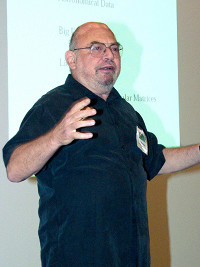
\includegraphics[width=0.3\textwidth]{images/images_intro/Leo_Breiman.jpg}
%     \caption{The american statistician Leo Breiman (1928-2005) author of \textit{Classification and Regression Trees} (1984)}
%     \label{fig:leo-breiman}
% \end{figure}

\RestyleAlgo{ruled}
\SetKwComment{Comment}{}{}
\begin{algorithm}
    \KwData{Training data $\mathcal{E} = \{(\boldsymbol{x}_i, y_i)\}_{i=1}^N$ where $\boldsymbol{x}_i \in \mathcal{X} \subseteq \mathbb{R}^p$ and $y_i \in \mathcal{Y} = \{1, \ldots, K\}$}
    \KwResult{Decision tree $T$}
    
    \SetKwProg{Fn}{Function}{:}{}
    \SetKwFunction{BuildTree}{BuildTree}
    \SetKwFunction{BestSplit}{BestSplit}
    \SetKwFunction{Gini}{Gini}
    \SetKwFunction{MajorityClass}{MajorityClass}
    
    \Fn{\BuildTree{$\mathcal{E}$}}{
        \If{stopping criterion met}{
            \Return leaf node with prediction $y_l \leftarrow$ MajorityClass$(\{y_i\}_{i=1}^N)$
        }
        
        $(feature, threshold) \leftarrow$ BestSplit$(\mathcal{E})$ \\
        
        \If{no valid split found}{
            \Return leaf node with prediction $y_l \leftarrow$ MajorityClass$(\{y_i\}_{i=1}^N)$
        }
        
        Split data: $\mathcal{E}_{left} = \{(\boldsymbol{x}_i, y_i) \in \mathcal{E} : x_{ij} \leq v\}$ \\
        \hspace{2.5cm} $\mathcal{E}_{right} = \{(\boldsymbol{x}_i, y_i) \in \mathcal{E} : x_{ij} > v\}$ \\
        
        $left\_child \leftarrow$ BuildTree$(\mathcal{E}_{left})$ \\
        $right\_child \leftarrow$ BuildTree$(\mathcal{E}_{right})$ \\
        
        \Return internal node with test function $\mathbb{I}[x_{ij} \leq threshold]$ and children $(left\_child, right\_child)$
    }
    
    \Fn{\BestSplit{$\mathcal{E}$}}{
        $best\_gain \leftarrow 0$ \\
        $best\_feature \leftarrow None$ \\
        $best\_threshold \leftarrow None$ \\
        
        \For{each feature $j \in \{1, \ldots, p\}$}{
            \For{each unique value $v$ in $\{x_{ij} : (\boldsymbol{x}_i, y_i) \in \mathcal{E}\}$}{
                $\mathcal{Y}_{left} \leftarrow \{y_i : (\boldsymbol{x}_i, y_i) \in \mathcal{E}, x_{ij} \leq v\}$ \\
                $\mathcal{Y}_{right} \leftarrow \{y_i : (\boldsymbol{x}_i, y_i) \in \mathcal{E}, x_{ij} > v\}$ \\
                
                $gain \leftarrow$ Gini$(\{y_i\}_{i=1}^N) - \frac{|\mathcal{Y}_{left}|}{N}$Gini$(\mathcal{Y}_{left}) - \frac{|\mathcal{Y}_{right}|}{N}$Gini$(\mathcal{Y}_{right})$ \\
                
                \If{$gain > best\_gain$}{
                    $best\_gain \leftarrow gain$ \\
                    $best\_feature \leftarrow f$ \\
                    $best\_threshold \leftarrow v$ \\
                }
            }
        }
        \Return $(best\_feature, best\_threshold)$
    }
    
    \Fn{\Gini{$\mathcal{Y}$}}{
        \Return $1 - \sum_{k=1}^K \left(\frac{|\{y_i \in \mathcal{Y} : y_i = k\}|}{|\mathcal{Y}|}\right)^2$ \Comment{// Gini impurity}
    }
    
    \Return BuildTree$(\mathcal{E})$
    \caption{CART for decision tree induction to optimize the supervised learning objective~\ref{def:sl}}\label{alg:cart}
\end{algorithm}

\section{Markov decision processes and problems}
\begin{figure}
    \centering
    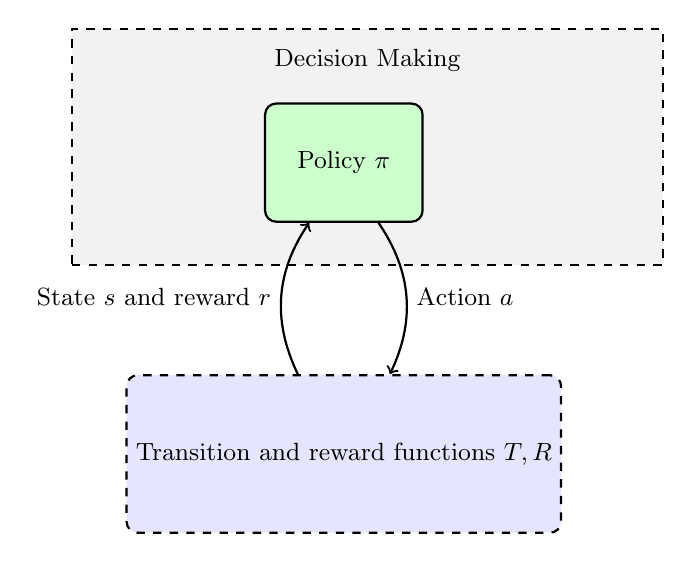
\begin{tikzpicture}[
        node distance=2.5cm,
        auto,
        thick,
        state/.style={circle, draw, fill=blue!20, minimum size=1.5cm, text centered},
        environment/.style={rectangle, draw, dashed, fill=blue!10, rounded corners, minimum width=4cm, minimum height=2cm, text centered},
        agent/.style={rectangle, draw, fill=orange!20, rounded corners, minimum width=2cm, minimum height=1.5cm, text centered},
        robot/.style={rectangle, draw, fill=green!20, rounded corners, minimum width=2cm, minimum height=1.5cm, text centered},
        decision_box/.style={rectangle, draw, dashed, fill=gray!10, minimum width=7.5cm, minimum height=3cm, text centered},
        arrow/.style={->, thick, bend left=15},
        arrow_decision/.style={->, dashed, bend left=15}
    ]
        
        % Decision Making Box
        \node[decision_box] (decision_box) at (0.3,3.4) {};
        \node at (0.3,4.5) {\small{Decision Making}};
        
        % Robot (AI)
        \node[robot] (robot) at (0,3.2) {\small{Policy $\pi$}};
        
        
        % Environment (Patient)
        \node[environment] (environment) at (0,-0.5) {\small{Transition and reward functions $T, R$}};
        
        % Arrows
        \draw[arrow] (environment) to[bend left=30] node[left] {\small{State $s$ and reward $r$}} (robot);
        \draw[arrow] (robot) to[bend left=30] node[right] {\small{Action $a$}} (environment);
        
    \end{tikzpicture}
    \caption{Markov decision process}
    \label{fig:MDP}
\end{figure}

Markov decision processes (MDPs) were first introduced in the 1950s by Richard Bellman~\cite{Bellman}.
Informally, an MDP models how an agent acts over time to achieve a goal. 
At every time step, the agent observes its current state (e.g., patient weight and tumor size) and takes an action (e.g., administers a certain amount of chemotherapy).
The agent receives a reward that helps evaluate the quality of the action with respect to the goal (e.g., tumor size decreases when the objective is to cure cancer).
Finally, the agent transitions to a new state (e.g., the updated patient state) and repeats this process over time. 
Following Martin L. Puterman's book on MDPs\cite{puterman}, we formally define:
\begin{definition}[Markov decision process]\label{def:mdp} An MDP is a tuple $\mathcal{M} = \langle S, A, R, T, T_0 \rangle$ where:
\begin{itemize}
\item $S$ is a finite set of states representing all possible configurations of the environment.
\item $A$ is a finite set of actions available to the agent.
\item $R: S \times A \rightarrow \mathbb{R}$ is a deterministic reward function that assigns a real-valued reward to each state-action pair. While in general reward functions are often stochastic, in this manuscript we focus deterministic ones without loss of generality.
\item $T: S \times A \rightarrow \Delta(S)$ is the transition function that maps state-action pairs to probability distributions over next states, where $\Delta(S)$ denotes a probability distribution over $S$.
\item $T_0 \in \Delta(S)$ is the initial distribution over states.
\end{itemize}
\end{definition}

Informally, we would like to act in an MDP so that we obtain as much reward as possible over time.
For example, in cancer treatment, the best outcome is to eliminate the patient's tumor as quickly as possible.
We can formally define this objective, that we call the reinforcement learning objective, as follows:

\begin{definition}[Reinforcement learning objective]\label{def:mdp-obj} Given an MDP $\mathcal{M}=\langle S, A, R, T, T_0 \rangle$ (cf. definition~\ref{def:mdp}), the goal of reinforcement learning for sequential decision making is to find a model, also known as a policy, $\pi: S \rightarrow A$ that maximizes the expected discounted sum of rewards:
$$J(\pi) = \mathbb{E}\left[\sum_{t=0}^{\infty} \gamma^t R(s_t, a_t) \mid s_0 \sim T_0, a_t = \pi(s_t), s_{t+1} \sim T(s_t, a_t)\right]$$
where $0< \gamma\leq 1$ is the discount factor that controls the trade-off between immediate and future rewards.
\end{definition}

Algorithms presented in this manuscript aim to find an optimal policy $\pi^\star \in\underset{\pi}{\operatorname{argmax}}J(\pi)$ that maximizes the above reinforcement learning (RL) objective.

\subsection{Example: a grid world MDP}
\begin{figure}
    \centering
    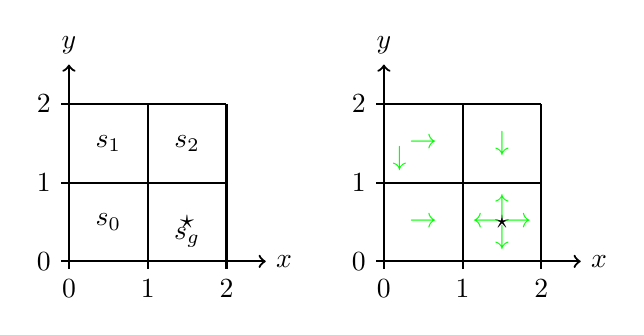
\begin{tikzpicture}
        \tikzstyle{grid}=[draw, thick, fill=gray!10]
        
        % Draw grid
        \draw[grid] (0,0) grid (2,2);
        
        % Add axes
        \draw[thick, ->] (0,0) -- (2.5,0) node[right] {$x$};
        \draw[thick, ->] (0,0) -- (0,2.5) node[above] {$y$};
        
        % Add tick marks and labels
        \foreach \x in {0,1,2} {
            \draw[thick] (\x,0) -- (\x,-0.1) node[below] {$\x$};
        }
        \foreach \y in {0,1,2} {
            \draw[thick] (0,\y) -- (-0.1,\y) node[left] {$\y$};
        }
        
        % Add state labels clockwise from bottom left
        \node at (0.5,0.5) {$s_0$};
        \node at (1.5,0.5) {$\star$};
        \node at (1.5,0.3) {$s_g$};
        \node at (1.5,1.5) {$s_2$};
        \node at (0.5,1.5) {$s_1$};


        % Draw grid
        \draw[grid] (4,0) grid (6,2);
        
        % Add axes
        \draw[thick, ->] (4,0) -- (6.5,0) node[right] {$x$};
        \draw[thick, ->] (4,0) -- (4,2.5) node[above] {$y$};
        
        % Add tick marks and labels
        \draw[thick] (4,0) -- (4,-0.1) node[below] {$0$};
        \draw[thick] (5,0) -- (5,-0.1) node[below] {$1$};
        \draw[thick] (6,0) -- (6,-0.1) node[below] {$2$};
        

        \foreach \y in {0,1,2} {
            \draw[thick] (4,\y) -- (3.9,\y) node[left] {$\y$};
        }
        
        % Add state labels clockwise from bottom left
        \node at (4.5,0.5) {{\color{green} $\rightarrow$}};
        \node at (5.5,0.5) {$\star$};
        \node at (5.5,0.7) {{\color{green} $\uparrow$}};
        \node at (5.5,0.3) {{\color{green} $\downarrow$}};
        \node at (5.7,0.5) {{\color{green} $\rightarrow$}};
        \node at (5.3,0.5) {{\color{green} $\leftarrow$}};
        \node at (5.5,1.5) {{\color{green} $\downarrow$}};
        \node at (4.2,1.3) {{\color{green} $\downarrow$}};
        \node at (4.5,1.5) {{\color{green} $\rightarrow$}};
    \end{tikzpicture}
    \caption{A grid world MDP (left) and optimal actions w.r.t. the objective~\ref{def:mdp-obj} (right).}\label{example:grid}
    \end{figure}

In figure~\ref{example:grid}, we present a very simple MDP (cf. definition~\ref{def:mdp}).
This MDP is essentially a grid where the starting state is chosen at random and the goal is to reach the bottom-right cell as fast as possible in order to maximize the RL objective (cf. definition~\ref{def:mdp-obj}).
The state space is discrete with state labels representing 2D-coordinates.
The actions are to move up, left, right, or down. 
The bottom-right cell gives reward 1 and is an absorbing state, i.e., once in the state, the MDP stays in this state forever.
Other states give reward 0 and are not absorbing.
The optimal actions that get to the goal as fast as possible in every state (cell) are presented in green in figure~\ref{example:grid}.

Next we present the tools to find solutions to MDPs and compute such optimal policies.

\section{Exact solutions for Markov decision problems}\label{sec:values}
We begin with the planning setting in which the MDP transitions and rewards (cf. definition~\ref{def:mdp}) are known. 
Leveraging the Markov property, one can use dynamic programming~\cite{Bellman} to compute optimal policies with respect to the RL objective (cf. definition~\ref{def:mdp-obj}).
Algorithms based on dynamic programming use the notion of \textit{value} of states and actions:
\begin{definition}[Value of a state]\label{def:vs} 
    In an MDP $\mathcal{M}$ (cf. definition~\ref{def:mdp}), the value of a state $s\in S$ under policy $\pi$ is the expected discounted sum of rewards starting from state $s$ and following policy $\pi$:
    $$V^\pi(s) = \mathbb{E}\left[\sum_{t=0}^{\infty} \gamma^t R(s_t, a_t) \mid s_0 = s, a_t = \pi(s_t), s_{t+1} \sim T(s_t, a_t)\right]$$
    Applying the Markov property gives a recursive definition of the value of $s$ under policy $\pi$:
    $$V^\pi(s) = R(s,\pi(s)) + \gamma \mathbb{E}\left[V^\pi(s') | s'\sim T(s, \pi(s))\right]$$
\end{definition}
\begin{definition}[Optimal value of a state] The optimal value of a state $s\in S$, $V^\star(s)$, is the value of state $s$ when following the optimal policy $\pi^{\star}$ (the policy that maximizes the RL objective (\ref{def:mdp-obj})).
    $$V^{\star}(s) = V^{\pi^{\star}}(s)$$
\end{definition}
\begin{definition}[Optimal value of a state–action pair]\label{def:qvalues} The optimal value of a state–action pair $(s,a)\in S\times A$, $Q^\star(s,a)$, is the value when taking action $a$ in state $s$ and then following the optimal policy.
    $$Q^{\star}(s,a) = R(s, a) + \gamma\mathbb{E}\left[V^{\star}(s') | s'\sim T(s, a)\right]$$
\end{definition}

The well-known value iteration (\cite{sutton}, cf. algorithm~\ref{alg:value-iteration}), computes the values of states $\V^{\star}(s)$ with respect to the policy $\pi^{\star}$ maximizing the RL objective (\ref{def:mdp-obj}). 

\RestyleAlgo{ruled}
\SetKwComment{Comment}{}{}
\begin{algorithm}
    \KwData{MDP $\mathcal{M} = \langle S, A, R, T, T_0 \rangle$}
    \KwResult{Optimal values $V^{\star}$ and optimal policy $\pi^*$}
    Initialize $V(s) = 0$ for all $s \in S$ \\
    \Repeat{Convergence}{
        \For{each state $s \in S$}{
            $v \leftarrow V(s)$ \\
            $V(s) \leftarrow \max_a \left[ R(s,a) + \gamma \sum_{s' \in S} T(s,a,s') V(s') \right]$ \Comment{// Bellman optimality update}
        }
    }
    \For{each state $s \in S$}{
        $\pi^*(s) \leftarrow \operatorname{argmax}_a \left[ R(s,a) + \gamma \mathbb{E}\left[V(s')|s'\sim T(s, a)\right]\right]$ \Comment{// Extract optimal policy}
    }
    \caption{Value iteration}\label{alg:value-iteration}
\end{algorithm}

More realistically, neither the transition function $T$ nor the reward function $R$ of the MDP are known, e.g. the doctor cannot \textbf{know} how the tumor and the patient's health will change after a dose of chemotherapy, but can only \textbf{observe} the change.
This distinction in available information parallels the distinction between dynamic programming and reinforcement learning, described next. 

\section{Reinforcement learning of approximate solutions to MDPs}\label{sec:rl}
When the MDP transition function and reward function are unknown, one can use reinforcement learning algorithms--also known as agents--to learn values or policies maximizing the RL objective (cf. definition~\ref{def:mdp-obj}). 
% \begin{figure}
%     \centering
%     \begin{subfigure}[b]{0.22\textwidth}
%         \centering
%         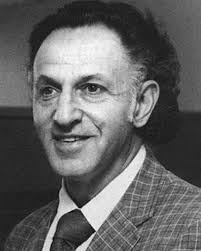
\includegraphics[width=0.7\textwidth]{images/images_intro/bellman.jpeg}
%         \caption{R. Bellman}
%     \end{subfigure}
%     \hfill
%     \begin{subfigure}[b]{0.22\textwidth}
%         \centering
%         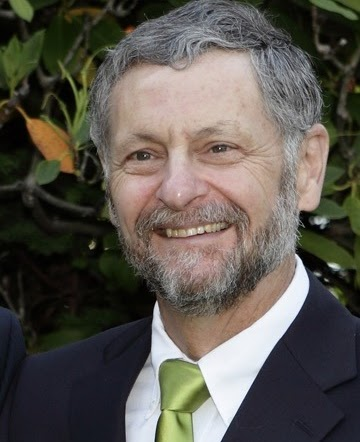
\includegraphics[width=0.7\textwidth]{images/images_intro/puterman.jpg}
%         \caption{M.L. Puterman}
%     \end{subfigure}
%     \hfill
%     \begin{subfigure}[b]{0.22\textwidth}
%         \centering
%         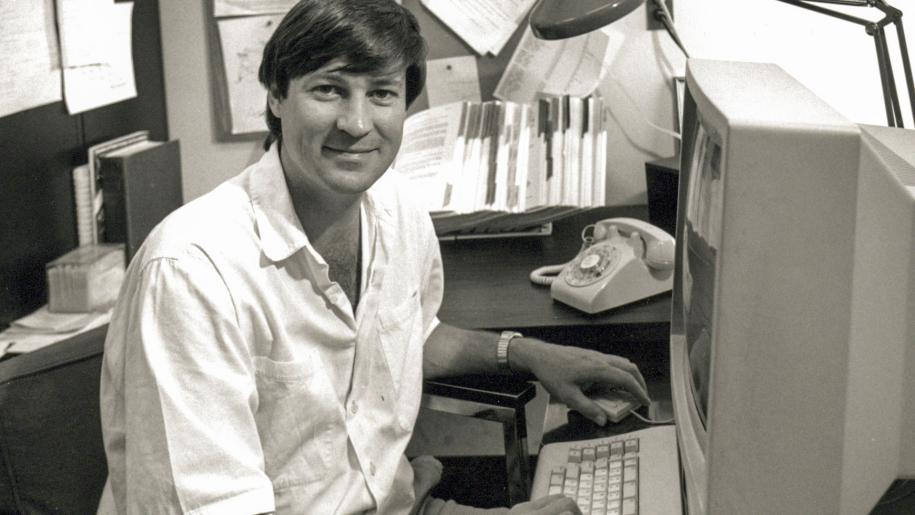
\includegraphics[width=1.2\textwidth]{images/images_intro/Barto_1982_umass_amherst.jpg}
%         \caption{A. Barto}
%     \end{subfigure}
%     \hfill
%     \begin{subfigure}[b]{0.22\textwidth}
%         \centering
%         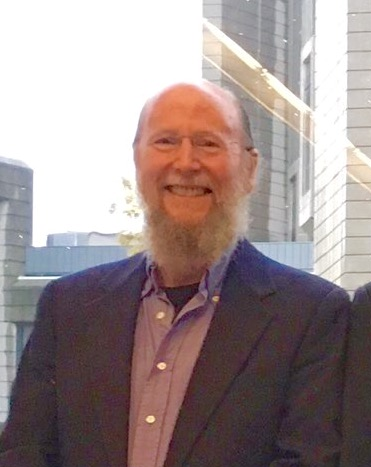
\includegraphics[width=0.67\textwidth]{images/images_intro/sutton.jpg}
%         \caption{R. Sutton}
%     \end{subfigure}
%        \caption{The godfathers of sequential decision making. Andrew Barto and Richard Sutton are the ACM Turing Prize 2024 laureate and share an advisor advisee relationship.}
%        \label{fig:rl-pioneers}
% \end{figure}

Reinforcement learning algorithms popularized by Richard Sutton~\cite{sutton} don't \textbf{compute} an optimal policy but rather \textbf{learn} an approximate one based on sequences of transitions $(s_t, a_t, r_t, s_{t+1})_t$.
RL algorithms usually fall into two categories: value-based~\cite{sutton} and policy search~\cite{pg_sutton}.
Examples of these approaches are shown in algorithms~\ref{alg:qlearning},~\ref{alg:sarsa} and~\ref{alg:reinforce}.
Q-learning and Sarsa compute an approximation of $Q^{\star}$ (cf. definition~\ref{def:qvalues}) using temporal difference learning~\cite{sutton}. Q-learning is \textit{off-policy}: it collects new transitions with a random policy, e.g. epsilon-greedy. Sarsa is \textit{on-policy}: it collects new transitions greedily w.r.t. the current Q-values estimates.
Policy gradient algorithms~\cite{pg_sutton} leverage the policy gradient theorem to approximate $\pi^{\star}$.

Q-learning, Sarsa, and policy gradients algorithms are known to converge to the optimal value or (locally) optimal policy under some conditions.
There are many other ways to learn policies such as simple random search~\cite{random-search} or model-based reinforcement learning that estimates MDP transitions and rewards before applying e.g. value iteration~\cite{ucbvi}. 
Those RL algorithms--also known as tabular RL because they represent policies as tables with $|S|\times |A|$ entries--is limited to small state spaces.
To scale to large state spaces, it is common to use a neural network to represent policies or values~\cite{tdgammon}.
In the next section, we present deep reinforcement learning algorithms designed specifically for neural networks.
\RestyleAlgo{ruled}
\SetKwComment{Comment}{}{}
\begin{algorithm}
    \KwData{MDP $\mathcal{M} = \langle S, A, R, T, T_0 \rangle$, learning rate $\alpha$, exploration rate $\epsilon$}
    \KwResult{Policy $\pi$}
    Initialize $Q(s,a) = 0$ for all $s \in S, a \in A$ \\
    Initialize state $s_0 \sim T_0$ \\
    \For{each step $t$}{
        Choose action $a_t$ using e.g. $\epsilon$-greedy policy: $a_t = \operatorname{argmax}_a Q(s_t,a)$ with prob. $1-\epsilon$ \\
        Take action $a_t$, observe $r_t = R(s_t,a_t)$ and $s_{t+1} \sim T(s_t,a_t)$ \\
        $Q(s_t,a_t) \leftarrow Q(s_t,a_t) + \alpha[r_t + \gamma \max_{a'} Q(s_{t+1},a') - Q(s_t,a_t)]$ \\
        $s_t \leftarrow s_{t+1}$ \\
    }
    $\pi(s) = \operatorname{argmax}_a Q(s,a)$ \Comment{// Extract greedy policy}
    \caption{Q-Learning}\label{alg:qlearning}
\end{algorithm}


\RestyleAlgo{ruled}
\SetKwComment{Comment}{}{}
\begin{algorithm}
    \KwData{MDP $\mathcal{M} = \langle S, A, R, T, T_0 \rangle$, learning rate $\alpha$, exploration rate $\epsilon$}
    \KwResult{Policy $\pi$}
    Initialize $Q(s,a) = 0$ for all $s \in S, a \in A$ \\
    Initialize state $s_0 \sim T_0$ \\
    Choose action $a_0$ using e.g. $\epsilon$-greedy: $a_0 = \operatorname{argmax}_a Q(s_0,a)$ with prob. $1-\epsilon$ \\
    \For{each step $t$}{
        Take action $a_t$, observe $r_t = R(s_t,a_t)$ and $s_{t+1} \sim T(s_t,a_t)$ \\
        Choose action $a_{t+1}$ using e.g. $\epsilon$-greedy: $a_{t+1} = \operatorname{argmax}_a Q(s_{t+1},a)$ with prob. $1-\epsilon$ \\
        $Q(s_t,a_t) \leftarrow Q(s_t,a_t) + \alpha[r_t + \gamma Q(s_{t+1},a_{t+1}) - Q(s_t,a_t)]$ \\
        $s_t \leftarrow s_{t+1}$ \\
        $a_t \leftarrow a_{t+1}$ \\
    }
    $\pi(s) = \operatorname{argmax}_a Q(s,a)$ \Comment{// Extract greedy policy}
    \caption{Sarsa}\label{alg:sarsa}
\end{algorithm}


\RestyleAlgo{ruled}
\SetKwComment{Comment}{}{}
\begin{algorithm}
    \KwData{MDP $\mathcal{M} = \langle S, A, R, T, T_0 \rangle$, learning rate $\alpha$, policy parameters $\theta$}
    \KwResult{Policy $\pi_\theta$}
    Initialize policy parameters $\theta$ \\
    \For{each episode}{
        Generate trajectory $\tau = (s_0, a_0, r_0, s_1, a_1, r_1, \ldots)$ following $\pi_\theta$ \\
        \For{each time step $t$ in trajectory}{
            $G_t \leftarrow \sum_{k=t}^{T} \gamma^{k-t} r_k$ \Comment{// Compute return}
            $\theta \leftarrow \theta + \alpha G_t \nabla_\theta \log \pi_\theta(a_t|s_t)$ \Comment{// Policy gradient update}
        }
    }
    \caption{Policy Gradient RL (REINFORCE)}\label{alg:reinforce}
\end{algorithm}


\section{Deep reinforcement learning for large or continuous state spaces}\label{sec:drl}

Reinforcement learning has also been successfully combined with function approximations to solve MDPs with large discrete state spaces or continuous state spaces ($S\subset \mathbb{R}^p$ in definition~\ref{def:mdp}).
In the rest of this manuscript, unless stated otherwise, we write $\boldsymbol{s}$ a state vector in a continuous state space\footnote{Note that discrete states can be one-hot encoded as state vectors in $\{0, 1\}^{|S|}$.}.

Deep Q-Networks (DQN)~\cite{dqn}, described in algorithm~\ref{alg:dqn} achieved super-human performance on a set of Atari games.
Authors successfully extended the Q-learning (algorithm~\ref{alg:qlearning}) to the function approximation setting by introducing target networks to mitigate distributional shift in the temporal difference error and replay buffer to increase sample efficiency.

Proximal Policy Optimization (PPO)~\cite{ppo}, described in algorithm~\ref{alg:ppo}, is an actor-critic algorithm~\cite{sutton} optimizing a neural network policy. 
In actor-critic algorithms, cumulative discounted rewards starting from a particular state, also known as \textit{the returns}, are also estimated with a neural network. 
PPO is known to work well in a variety of domains including robot control in simulation among others.

\begin{algorithm}
    \KwData{MDP $\mathcal{M} = \langle S, A, R, T, T_0 \rangle$, learning rate $\alpha$, exploration rate $\epsilon$, Q-network parameters $\theta$, update frequency $C$}
    \KwResult{Policy $\pi$}
    Initialize Q-network parameters $\theta$ and target network parameters $\theta^- = \theta$ \\
    Initialize replay buffer $\mathcal{B} = \emptyset$ \\
    \For{each episode}{
        Initialize state $s_0 \sim T_0$ \\
        \For{each step $t$}{
            Choose action $a_t$ using $\epsilon$-greedy: $a_t = \operatorname{argmax}_a Q_\theta(\boldsymbol{s}_t,a)$ with prob. $1-\epsilon$ \\
            Take action $a_t$, observe $r_t = R(s_t,a_t)$ and $\boldsymbol{s}_{t+1} \sim T(\boldsymbol{s}_t,a_t)$ \\
            Store transition $(\boldsymbol{s}_t, a_t, r_t, \boldsymbol{s}_{t+1})$ in $\mathcal{B}$ \\
            Sample random batch $(\boldsymbol{s}_i, a_i, r_i, \boldsymbol{s}_{i+1}) \sim \mathcal{B}$ \\
            $y_i = r_i + \gamma \max_{a'} Q_{\theta^-}(\boldsymbol{s}_{i+1}, a')$ \Comment{// Compute target}
            $\theta \leftarrow \theta - \alpha \nabla_\theta (Q_\theta(\boldsymbol{s}_i, a_i) - y_i)^2$ \Comment{// Update Q-network}
            \If{$t \bmod C = 0$}{
                $\theta^- \leftarrow \theta$ \Comment{// Update target network}
            }
            $\boldsymbol{s}_t \leftarrow \boldsymbol{s}_{t+1}$ \\
        }
    }
    $\pi(\boldsymbol{s}) = \operatorname{argmax}_a Q_\theta(\boldsymbol{s},a)$ \Comment{// Extract greedy policy}
    \caption{Deep Q-Network (DQN)}\label{alg:dqn}
\end{algorithm}


\begin{algorithm}
    \KwData{MDP $\mathcal{M} = \langle S, A, R, T, T_0 \rangle$, learning rate $\alpha$, policy parameters $\theta$, clipping parameter $\epsilon$, value function parameters $\phi$}
    \KwResult{Policy $\pi_\theta$}
    Initialize policy parameters $\theta$ and value function parameters $\phi$ \\
    \For{each episode}{
        Generate trajectory $\tau = (\boldsymbol{s}_0, a_0, r_0, \boldsymbol{s}_1, a_1, r_1, \ldots)$ following $\pi_\theta$ \\
        \For{each time step $t$ in trajectory}{
            $G_t \leftarrow \sum_{k=t}^{T} \gamma^{k-t} r_k$ \Comment{// Compute return}
            $A_t \leftarrow G_t - V_\phi(\boldsymbol{s}_t)$ \Comment{// Compute advantage}
            $r_t(\theta) \leftarrow \frac{\pi_\theta(a_t|\boldsymbol{s}_t)}{\pi_{\theta_{old}}(a_t|\boldsymbol{s}_t)}$ \Comment{// Compute probability ratio}
            $L^{CLIP}_t \leftarrow \min(r_t(\theta) A_t, \text{clip}(r_t(\theta), 1-\epsilon, 1+\epsilon) A_t)$ \Comment{// Clipped objective}
            $\theta \leftarrow \theta + \alpha \nabla_\theta L^{CLIP}_t$ \Comment{// Policy update}
            $\phi \leftarrow \phi + \alpha \nabla_\phi (G_t - V_\phi(\boldsymbol{s}_t))^2$ \Comment{// Value function update}
        }
        $\theta_{old} \leftarrow \theta$ \Comment{// Update old policy}
    }
    \caption{Proximal Policy Optimization (PPO)}\label{alg:ppo}
\end{algorithm}
In this manuscript we study those two deep reinforcement learning algorithms for various problems.

\section{Imitation learning: a baseline (indirect) interpretable reinforcement learning method}\label{sec:imit}

Unlike PPO or DQN for neural networks, there does not exist an algorithm that trains decision tree policies to optimize the RL objective (cf. definition~\ref{def:mdp-obj}).
In fact, we will show in the first part of the manuscript that training decision trees that optimize the RL objective is very difficult.

Hence, many interpretable reinforcement learning approaches first train a neural network policy--also called an expert policy--to optimize the RL objective (cf. definition~\ref{def:mdp-obj}) using e.g. PPO, and then fit a student policy such as a decision tree using CART (cf. algorithm~\ref{alg:cart}) to optimize the supervised learning objective (cf. definition~\ref{def:sl}) with the neural policy actions as targets.
This approach is known as imitation learning and is essentially training a student policy to optimize the objective:

\begin{definition}[Imitation learning objective]\label{def:il}
Given an MDP $\mathcal{M}$ (cf. definition~\ref{def:mdp}) expert policy $\pi^*$ and a policy class $\Pi$, e.g. decision trees of depth at most 3, the imitation learning objective is to find a student policy $\hat{\pi} \in \Pi$ that minimizes the expected action disagreement with the expert:
\begin{equation}
IL(\pi) &=  \mathbb{E}_{\boldsymbol{s} \sim \rho(\boldsymbol{s})} \left[ \mathcal{L}(\pi(\boldsymbol{s}), \pi^*(\boldsymbol{s})) \right]
\end{equation}
where $\rho(\boldsymbol{s})$ is the state distribution in $\mathcal{M}$ induced by the student policy $\pi$ and $\mathcal{L}$ is a loss function measuring the disagreement between the student policy's action $\pi(s)$ and the expert's action $\pi^*(s)$.
\end{definition}

There are two main imitation learning methods used for interpretable reinforcement learning.
Dagger (\cite{PIRL}; algorithm~\ref{alg:dagger}) is a straightforward way to fit a decision tree policy to optimize the imitation learning objective\ref{def:il}.
VIPER (\cite{viper}; algorithm~\ref{alg:viper}) was designed specifically for interpretable reinforcement learning.
VIPER re-weights the transitions collected by the neural network expert by a function of the state-action value (cf. definition~\ref{sec:values}).
The authors of VIPER showed that decision tree policies fitted with VIPER tend to have the same RL objective value as Dagger trees while being more interpretable (shallower or with fewer nodes) and sometimes outperform Dagger trees.
Dagger and VIPER are two strong baselines for decision tree learning in MDPs, but they optimize a surrogate objective only, even though in practice the resulting decision tree policies often achieve high RL objective value.
We use these two algorithms extensively throughout the manuscript.
Next we show how to learn a decision tree policy for the example MDP (cf. figure~\ref{example:grid}).

\begin{algorithm}
    \caption{Dagger}\label{alg:dagger}
    \KwIn{Expert policy $\pi^*$, MDP $M$, policy class $\Pi$}
    \KwOut{Fitted student policy $\hat{\pi}_i$}
    
    % Initialize empty dataset and initial policy
    Initialize dataset $\mathcal{D} \gets \emptyset$\;
    Initialize $\hat{\pi}_1$ arbitrarily from $\Pi$\;
    
    \For{$i \gets 1$ \KwTo $N$}{
        % Create mixed policy using expert and current policy
        \lIf{i = 1}{
        $\hat{\pi} \gets \pi^*$\
        }
          \lElse{
            $\pi_i \gets \hat{\pi}_i$
          } \label{alg:expert-or-student}
        % Collect data using mixed policy
        Sample transitions from $M$ using $\hat{\pi}$\;
        % Get expert actions for visited states
        Collect dataset $\mathcal{D}_i \gets \{ (\boldsymbol{s}, \pi^*(\boldsymbol{s})) \}$ of states visited by $\hat{\pi}$\;
        
        % Aggregate datasets
        $\mathcal{D} \gets \mathcal{D} \cup \mathcal{D}_i$\;
        
        % Train new policy
       Fit classifier/regressor $\hat{\pi}_{i+1}$ on $\mathcal{D}$\;\label{alg:fit}
    }
    \Return $\hat{\pi}$\;
    \end{algorithm}


    \begin{algorithm}
        \caption{VIPER}\label{alg:viper}
        \KwIn{Expert policy $\pi^*$, Expert Q-function $Q^*$, MDP $M$, policy class $\Pi$}
        \KwOut{Fitted student policy $\hat{\pi}_i$}
        
        % Initialize empty dataset and initial policy
        Initialize dataset $\mathcal{D} \gets \emptyset$\;
        Initialize $\hat{\pi}_1$ arbitrarily from $\Pi$\;
        
        \For{$i \gets 1$ \KwTo $N$}{
            % Create mixed policy using expert and current policy
            \lIf{i = 1}{
            $\hat{\pi} \gets \pi^*$\
            }
              \lElse{
                $\pi_i \gets \hat{\pi}_i$
              } \label{alg:expert-or-student}
            % Collect data using mixed policy
            Sample transitions from $M$ using $\hat{\pi}$\;
            % Get expert actions for visited states
            Weight each transition by $w(\boldsymbol{s}) \gets V^{\pi^*}(\boldsymbol{s}) - \min_a Q^{\pi^*}(\boldsymbol{s}, a)$\;
            Collect dataset $\mathcal{D}_i \gets \{ (\boldsymbol{s}, \pi^*(\boldsymbol{s}), w(\boldsymbol{s})) \}$ of states visited by $\hat{\pi}$\;            
            % Aggregate datasets
            $\mathcal{D} \gets \mathcal{D} \cup \mathcal{D}_i$\;
            
            % Train new policy
           Fit classifier/regressor $\hat{\pi}_{i+1}$ on the weighted dataset $\mathcal{D}$\;\label{alg:fit}
        }
        \Return $\hat{\pi}$\;
        \end{algorithm}

\section{Your first decision tree policy}\label{sec:limits-il}
Now the reader should know how to train decision tree classifiers or regressors for supervised learning using CART (cf. section~\ref{sec:sl}).
The reader should also know what an MDP is and how to compute or learn policies that optimize the RL objective (cf. definition~\ref{def:mdp-obj}) with (deep) reinforcement learning (cf. section~\ref{sec:drl}).
Finally, the reader should now know how to obtain a decision tree policy for an MDP through imitation learning (cf. definition~\ref{def:il}) by first using RL to get an expert policy and then fitting a decision tree to optimize the supervised learning objective, using the expert actions as labels.

In this section we present the first decision tree policies of this manuscript obtained using Dagger or VIPER after learning an expert Q-function for the grid world MDP of example (\ref{example:grid}) using Q-learning (cf. algorithm~\ref{alg:qlearning}).
Recall the optimal policies for the grid world, taking the green actions in each state in figure~\ref{example:grid}. 
Among the optimal policies, the ones that go left or up in the goal state can be problematic for imitation learning algorithms.
Indeed, we know that for this grid world MDP there exists decision tree policies with a very good interpretability-performance trade-off: depth-1 decision trees that are optimal w.r.t. the RL objective.
One could even say that those trees have the \textit{optimal} interpretability-performance trade-off because they are the shortest trees that are optimal w.r.t. the RL objective.

In figure~\ref{fig:trees-intro}, we present a depth-1 decision tree policy that is optimal w.r.t. the RL objective and a depth-1 tree that is sub-optimal.
The other optimal depth-1 tree is to go right when $y\leq 1$ and down otherwise.
Indeed, figure~\ref{fig:objectives} shows that the optimal depth-1 tree achieves exactly the same RL objective value as the optimal policies from figure~\ref{example:grid}, independently of the discount factor $\gamma$.

Now a fair question is: can Dagger or VIPER learn such an optimal depth-1 tree given access to an expert optimal policy from figure~\ref{example:grid}?

We start by running the standard Q-learning algorithm as presented in algorithm~\ref{alg:qlearning} with $\epsilon=0.3$, $\alpha=0.1$ over 10,000 time steps.
The careful reader might wonder how ties are broken in the $\operatorname{argmax}$ operation from algorithm~\ref{alg:qlearning}.
While Sutton and Barto break ties by index value in their book~\cite{sutton} (the greedy action is the $\operatorname{argmax}$ action with smallest index), we show that the choice of tie-breaking greatly influences the performance of subsequent imitation learning algorithms.
Indeed, depending on how actions are ordered in practice, Q-learning may be biased toward some optimal policies rather than others.
While this does not matter for one who just wants to find an optimal policy, in our example of finding the optimal depth-1 decision tree policy, it matters \textit{a lot}.

In the left plot of figure~\ref{fig:ql-il}, we see that Q-learning, independently of how ties are broken, consistently converges to an optimal policy over 100 runs (random seeds).
However, in the right plot of figure~\ref{fig:ql-il}, where we plot the proportion over 100 runs of optimal decision trees returned by Dagger or VIPER at different stages of Q-learning, we observe that imitating the optimal policy obtained by breaking ties at random consistently yields more optimal trees than breaking ties by indices.
What actually happens is that the most likely output of Q-learning when ties are broken by indices is the optimal policy that goes left in the goal state,
which cannot be perfectly represented by a depth-1 decision tree, because there are three different actions taken and a binary tree of depth $D=1$ can only map to $2^D=2$ labels.

This short experiment shows that imitation learning approaches can sometimes be very bad at learning decision tree policies with good interpretability-performance trade-offs for very simple MDPs. 
Despite VIPER almost always finding the optimal depth-1 decision tree policy in terms of the RL objective when ties are broken at random, we have shed light on the sub-optimality of indirect approaches such as imitation learning.
This motivates the study of direct approaches (cf. figure~\ref{fig:direct-vs-indirect-methods}) to directly search for policies with good interpretability-performance trade-offs with respect to the original RL objective.
Next, we present the outline of the thesis.

\begin{figure}
    \centering
    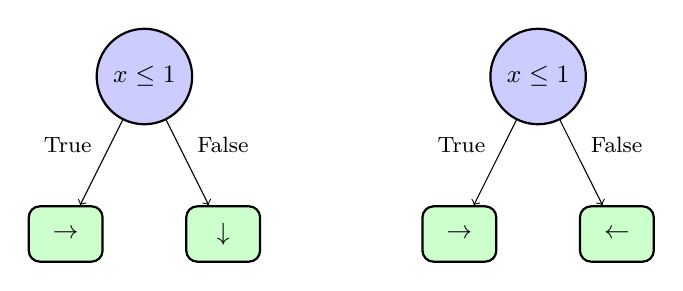
\begin{tikzpicture}[
        decision/.style={circle, draw, thick, fill=blue!20, text width=2.5em, text centered, minimum height=2.5em, font=\small},
        leaf/.style={rectangle, draw, thick, fill=green!20, text width=2em, text centered, rounded corners, minimum height=2em, font=\small},
        edge_label/.style={font=\footnotesize, midway}
    ]
        % Tree 4: if x <= 0.5 move right else move left
        \node[decision] (tree4_root) at (10,2) {$x \leq 1$};
        \node[leaf] (tree4_right) at (9,0) {$\rightarrow$};
        \node[leaf] (tree4_left) at (11,0) {$\leftarrow$};
        \draw[->] (tree4_root) -- (tree4_right) node[edge_label, above left] {True};
        \draw[->] (tree4_root) -- (tree4_left) node[edge_label, above right] {False};
        \tikzstyle{grid}=[draw, thick, fill=gray!10]


        % Tree 4: if x <= 0.5 move right else move left
        \node[decision] (tree5_root) at (5,2) {$x \leq 1$};
        \node[leaf] (tree5_right) at (4,0) {$\rightarrow$};
        \node[leaf] (tree5_left) at (6,0) {$\downarrow$};
        \draw[->] (tree5_root) -- (tree5_right) node[edge_label, above left] {True};
        \draw[->] (tree5_root) -- (tree5_left) node[edge_label, above right] {False};
        \tikzstyle{grid}=[draw, thick, fill=gray!10]

    \end{tikzpicture}
    \caption{Left, an optimal depth-1 decision tree policy. On the right, a sub-optimal depth-1 decision tree policy.}\label{fig:trees-intro}
    \end{figure}

\begin{figure}
    \centering
    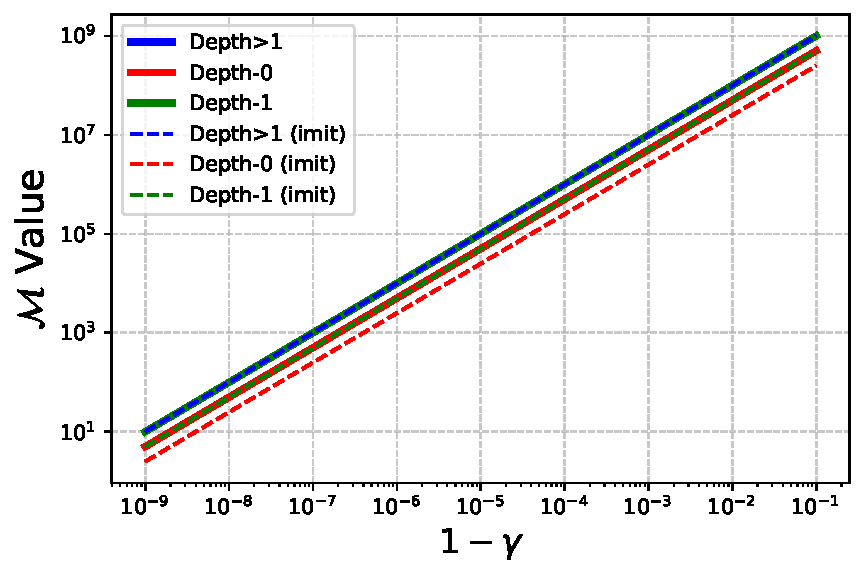
\includegraphics[width=0.5\textwidth]{images/images_part1/policy_values_comparison.pdf}
    \caption{The RL objective (\ref{def:mdp-obj}) values of the optimal policies from figure~\ref{example:grid} and of the decision tree policies from figure~\ref{fig:trees-intro}.}\label{fig:objectives}
\end{figure}

\begin{figure}
    \centering
    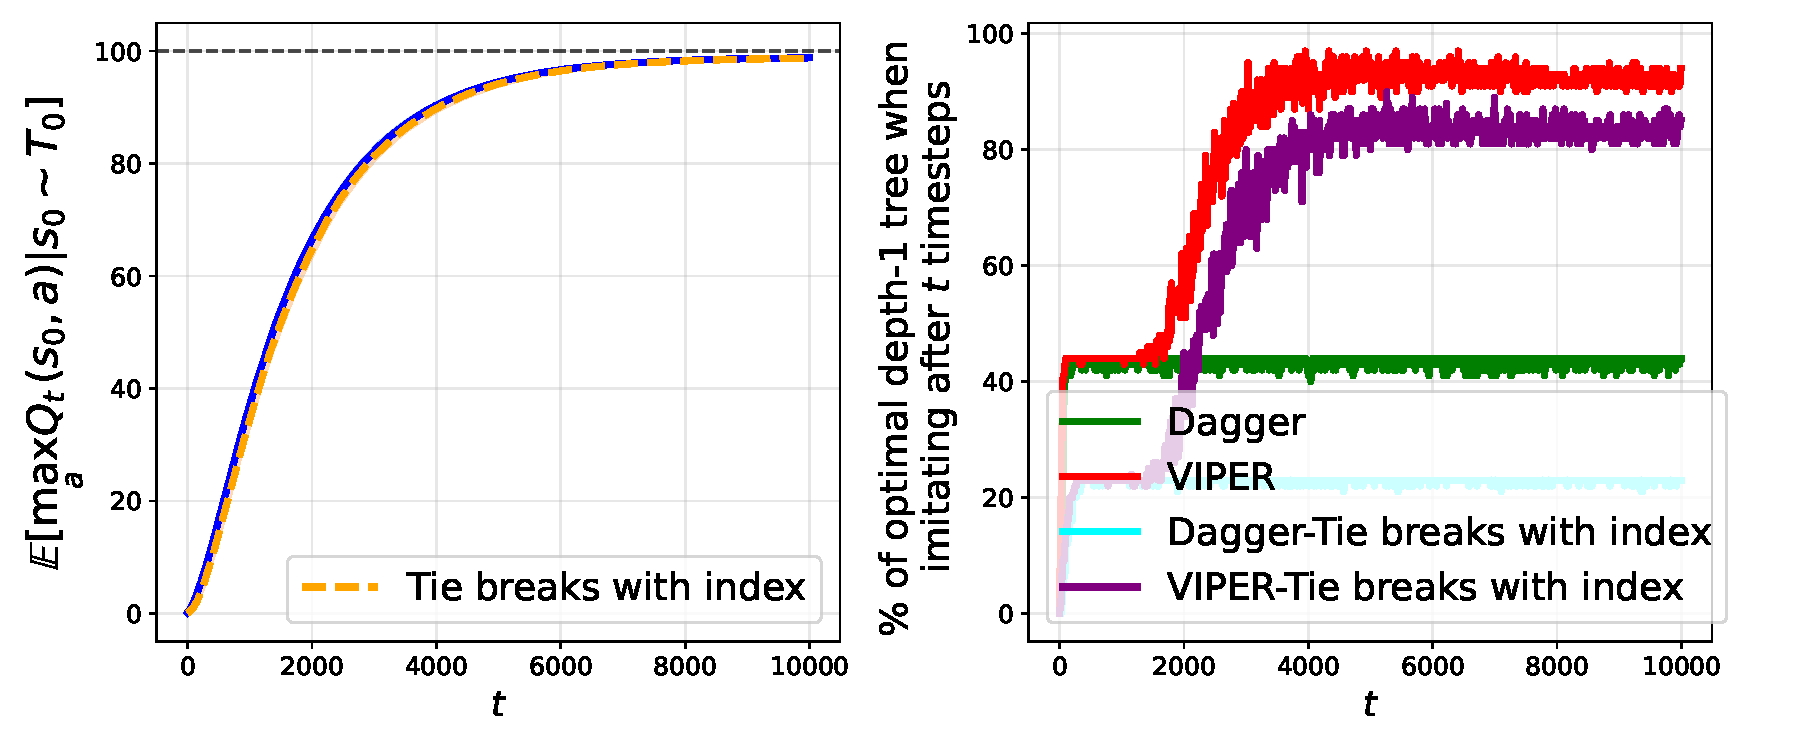
\includegraphics[width=1\textwidth]{images/images_part1/base_mdp.pdf}
    \caption{Left, sample complexity curve of Q-learning with default hyperparameters on the $2\times 2$ grid world MDP over 100 random seeds. Right, performance of indirect interpretable methods when imitating the greedy policy with a tree at different Q-learning stages.}\label{fig:ql-il}
\end{figure}

\section{Outline of the thesis}
Throughout our thesis, we make the assumption that constraining models (e.g. policies or classifiers) to be decision trees is enough for ensuring interpretability.
In this thesis we study different decision tree learning algorithms in different settings. 
In the first part of the manuscript, we show that direct decision tree learning methods (cf. figure~\ref{fig:direct-vs-indirect-methods}) struggle to find decision tree policies even for very simple sequential decision making problems.
For that, we first reproduce the work from~\cite{topin2021iterative} that presents a formalism for learning decision tree policies that optimize the RL objective (cf. definition~\ref{def:mdp-obj}) directly using reinforcement learning, and then make connections with hardness results from the partially observable MDPs (POMDPs) literature~\cite{POMDP,chap2}.
In the second part of the manuscript, we formulate decision tree induction for supervised learning as solving a sequential decision making problem.
By formalizing decision tree induction for the supervised learning objective (cf. definition~\ref{def:sl}) as solving an MDP (cf. definition~\ref{def:mdp}), we design novel algorithms that achieve very good performances.
In the last part of the text, we lift our assumption about decision trees being intrinsically interpretable and study other model classes.
In particular, we leverage the simplicity of indirect methods to imitate neural network experts with models from figure~\ref{fig:interpretability-performance-tradeoff} and perform a large-scale empirical study of the interpretability-performances trade-offs on various sequential decision making tasks.
% In Table~\ref{tab:summary-parts} we summarize the outline of this manuscript in terms of learning objective (~\ref{def:sl},~\ref{def:mdp-obj}, or~\ref{def:il}) and model class (figure~\ref{fig:interpretability-performance-tradeoff}).

% \begin{table}
%     \centering
%     \begin{tabular}{|l|c|c|c|c|}
%         \hline
%          & \textbf{Decision Trees} & \textbf{Linear} & \textbf{Ensembles} & \textbf{Neural Networks} \\
%         \hline
%         Supervised Learning & Part II &  & Part II & Part II\\
%         \hline
%         Reinforcement Learning & Part I, III & Part III & & Part I, III \\
%         \hline
%         Imitation Learning & Part I, III & Part III & & Part III \\
%         \hline
%     \end{tabular}
%     \caption{Summary of objectives and model classes studied in this manuscript.}
%     \label{tab:summary-parts}
% \end{table}

We summarize our results as follows:

\begin{enumerate}
    \item Direct reinforcement learning of decision tree policies is hard because it involves POMDPs.
    \item One can use dynamic programming in MDPs to induce highly performing decision tree classifiers and regressors.
    \item In practice, controlling MDPs with interpretable policies does not necessarily decrease performances.
\end{enumerate}

% \begin{figure}
%     \centering
%     \begin{tikzpicture}[
%         bubble/.style={rectangle, rounded corners=15pt, draw, thick, fill=blue!20, text width=3.5cm, text centered, minimum height=1.5cm, font=\small},
%         arrow/.style={->, thick},
%         label/.style={font=\footnotesize, text width=3cm, text centered}
%     ]
        
%         % Define the three vertices of the triangle
%         % Top bubble - chapter 1
%         \node[bubble] (ch1) at (0,4) {Part 1\\Direct learning of interpretable policies for MDPs};
        
%         % Bottom left bubble - chapter 2  
%         \node[bubble] (ch2) at (-4,0) {Part 2\\Supervised learning of decision tree classifiers with MDPs};
        
%         % Bottom right bubble - chapter 3
%         \node[bubble] (ch3) at (4,0) {Part 3\\Indirect learning of interpretable policies to compare different model classes};
        
%         % Arrow from chapter 1 to chapter 2
%         \draw[arrow] (ch1.south west) -- (ch2.north);
%         \node[label] at (-4.5,2.5) {Too difficult, let us assume uniform transitions};
        
%         % Arrow from chapter 1 to chapter 3  
%         \draw[arrow] (ch1.south east) -- (ch3.north);
%         \node[label] at (4.5,2.5) {Too difficult, let us use indirect approach};

%         % Arrow from chapter 1 to chapter 3  
%         \draw[arrow] (ch2.east) -- (ch3.west);
%         \node[label] at (0,1.1) {Use new decision tree induction to learn better interpretable policies};
        
        
%     \end{tikzpicture}
%     \caption{Thesis structure showing the progression from direct reinforcement learning of decision tree policies (chapter 1) to simplified approaches: supervised learning with uniform transitions (chapter 2) and indirect learning methods (chapter 3).}
%     \label{fig:thesis-outline}
% \end{figure}